%% LaTeX2e class for student theses
%%
%% Karlsruhe Institute of Technology
%% Institute of Information Security and Dependability
%% Software Design and Quality (SDQ)
%%
%% Dr.-Ing. Erik Burger
%% burger@kit.edu
%%
%% Version 1.6, 2024-06-07

\chapter{Implementation}
\label{ch:Implementation}

This chapter describes the implementation of the proposed features to the \LiSSAf to optimize classification prompts for fixed datasets.
As outlined in \autoref{ch:Approach}, the goal is to optimize prompts for a given set of \TLR tasks on a fixed dataset.
\Todo{Link to subsectsion in Approach, name features explicitly und ggf. auch auf die folgenden sections eingehen}
To achieve this goal, a new \promptoptimizer component is added to the \LiSSA pipeline.
This component can be combined with further optional \metric and \evaluator components to enable a flexible and reusable architecture.
\Todo{Unklar, das kennen wir ja noch nicht. Ggf. in erster subsecc zusammenhänge aufzeigen}
\autoref{fig:component_diagramm} provides an overview of the components involved in this implementation.

\begin{figure}
    \centering
    \includegraphics[width=\textwidth]{graphics/class_diagrams/components}
    \caption{Overview of the major new components involved in the implementation}
    \label{fig:component_diagramm}
\end{figure}

\section{Metric component}
\label{sec:impl:metric_component}
\Todo{Ggf. Scoring nenen um nicht mit Eval zu verwechseln}
The \metric component provides implementations for different metrics to score the quality of a prompt on a given set of tasks.
Metrics can be divided into two major categories.
Pointwise metrics will evaluate each \TL prediction and return a separate score for each.
\Todo{Pointwise nicht der beste Name, wird doch auch aggergeiert}
Scoring strategies for pointwise metrics are provided by the \scorer subcomponent.
The overall score can then be calculated by reducing the individual scores using a \reductor.
The \reductor subcomponent provides different strategies to reduce a collection of scores to a single value.
In contrast, global metrics will evaluate the entire set of \TL predictions at once and return a single score directly.
This is because they factor in relationships between different predictions, like whether the correct prediction is a true positive or a true negative.

The scores are cached using \LiSSAs built-in \cache component.

\begin{figure}
    \centering
    \fontsize{8}{10}\selectfont
    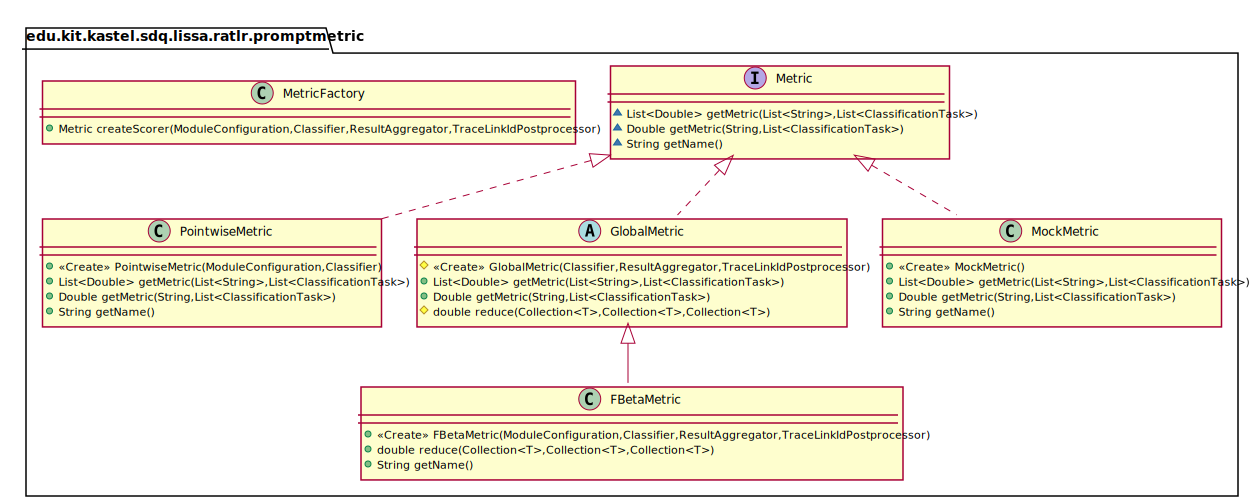
\includegraphics[width=\textwidth]{graphics/class_diagrams/metric}
    \caption{The new \metric component and its implementations}
    \label{fig:metric_component_diagramm}
\end{figure}

Currently, only the \fbeta metric is implemented as a global metric.
The beta parameter can be altered in the component configuration.
The pointwise metric implementation relies on the \method{Binary}\scorer and the \method{Mean}\reductor.
This is also portrayed in \autoref{fig:scorer_reductor_diagramm}.
The \method{Binary}\scorer will return a score of 1.0 for a correct prediction and 0.0 otherwise.
A correct prediction is defined as predicting a \TL for a pair of artifacts that actually has a \TL in the ground truth or not predicting a \TL for a pair of artifacts that does not have a \TL in the ground truth.
The \method{Mean}\reductor will then compute the mean of all individual scores to return a single value.


\begin{figure}
    \centering
    \fontsize{8}{10}\selectfont
    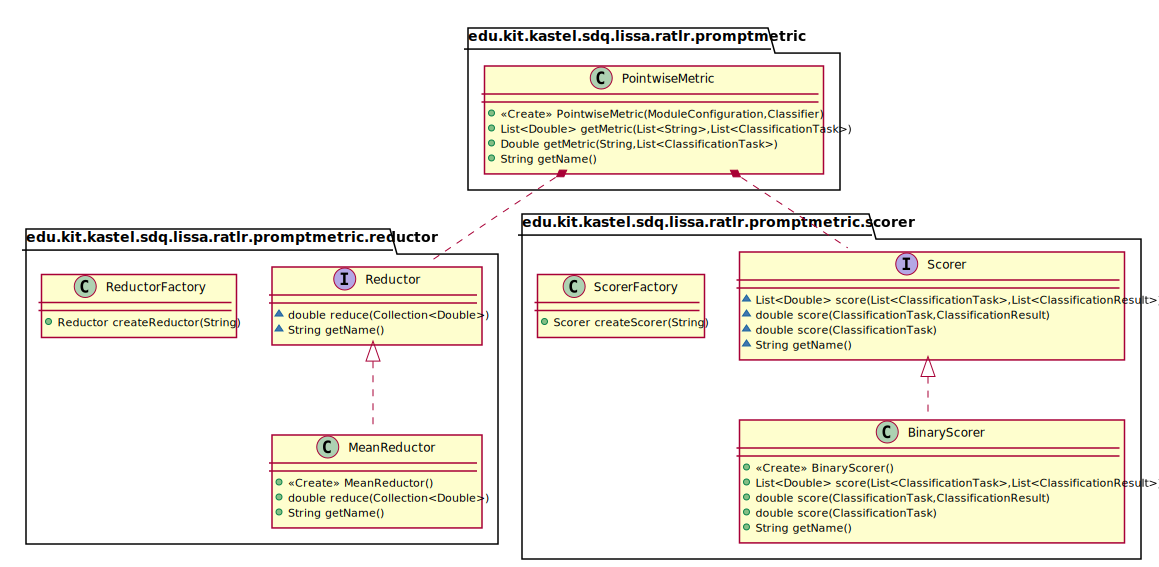
\includegraphics[width=\textwidth]{graphics/class_diagrams/pointwise_metric}
    \caption{The subcomponents utilized by the pointwise metric implementation}
    \label{fig:scorer_reductor_diagramm}
\end{figure}
\Todo{Was bringt mir \autoref{fig:scorer_reductor_diagramm} genau?}

\section{Evaluator component}
\label{sec:impl:evaluator_component}
\Todo{Ggf. ABlaufdiagramm statt UML. Nicht klar was das Modul macht}
The \evaluator component provides implementations to evaluate the quality of a prompt on a given set of tasks.
In contrast to the \metric component, the \evaluator will not use all tasks to compute the prompt score.
Instead, more complex sampling strategies can be used to select a subset of tasks.
This is especially useful for larger datasets, where evaluating all tasks would be too costly.
The \ucb bandit evaluator is the most noteworthy implementation.
It will use the \ucb algorithm to select a subset of tasks that are expected to provide the most information gain.
This is achieved by balancing exploration and exploitation.
The size of the subset can be configured in the component configuration.
The \ucb evaluator can be configured with a random seed to ensure reproducibility of results.

\begin{figure}
    \centering
    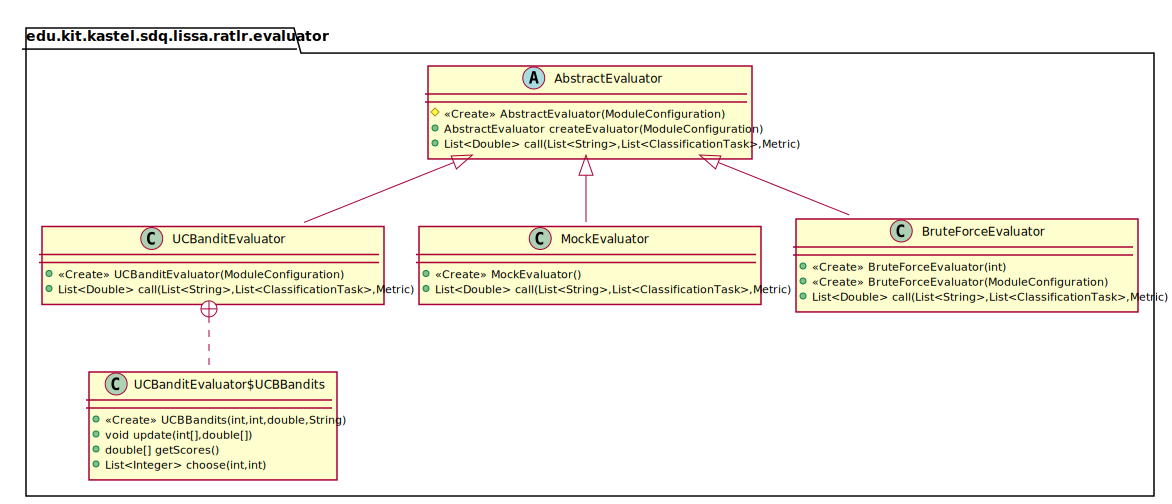
\includegraphics[width=\textwidth]{graphics/class_diagrams/evaluator}
    \caption{The new \evaluator component and its implementations}
    \label{fig:evaluator_component_diagramm}
\end{figure}

Other implementations seen in \autoref{fig:evaluator_component_diagramm} are the \method{BruteForceEvaluator}, which will use all tasks to evaluate the prompt.
The \method{MockEvaluator} is used for testing purposes and will return a fixed score.

\section{Prompt Optimizer component}
\label{sec:impl:prompt_optimizer_component}

The prompt optimizer component provides implementations for the actual prompt optimization.
Concrete objects will be instantiated with a set of configuration parameters, again following the format of the \LiSSAf.
A factory class is used to create the object based on the configuration.
Furthermore, the \metric and \evaluator components are provided to the respective constructors if required.
The \metric component is used to score the quality of a prompt on a given set of tasks.
The \evaluator component is used to select a subset of tasks to evaluate the prompt on.
This compoent is designed to be used in the \LiSSA evaluation pipeline after the preprocessing of artifacts into \elementstore's is completed.
These steps are already part of the existing \LiSSA framework for evaluation.
They are explained in more detail in \autoref{sec:foundations:lissa}.
\newcommand{\optimizermethod}{\method{optimize}}
\Todo{Check if this method is still named the same}
The only functionality required in the \promptoptimizer interface is the \optimizermethod method.
The \optimizermethod requires the source and target \elementstores created in the previous pipeline steps as arguments.
Using the retrieval strategy of the target \elementstore a set of candidate pairs of elements is created.
This set will also be referred to as the training data, on which the prompt will be optimized.

The prompt to be optimized is provided in the component configuration during the optimizers' instantiation.
The method will return the optimized prompt as a string.
When \promptoptimizer implementations utilize \classifiers, the training data or subsets will be passed on to the classification method.
Utilizing caching for the \LLM queries, which is implemented for \LiSSAs classifiers, the optimization is deterministic and reproducible.
All further implmentations should also be deterministic and reproducible.
Configuration parameters such as random seeds can be utilized.

\begin{figure}
    \centering
    \fontsize{8}{10}\selectfont
    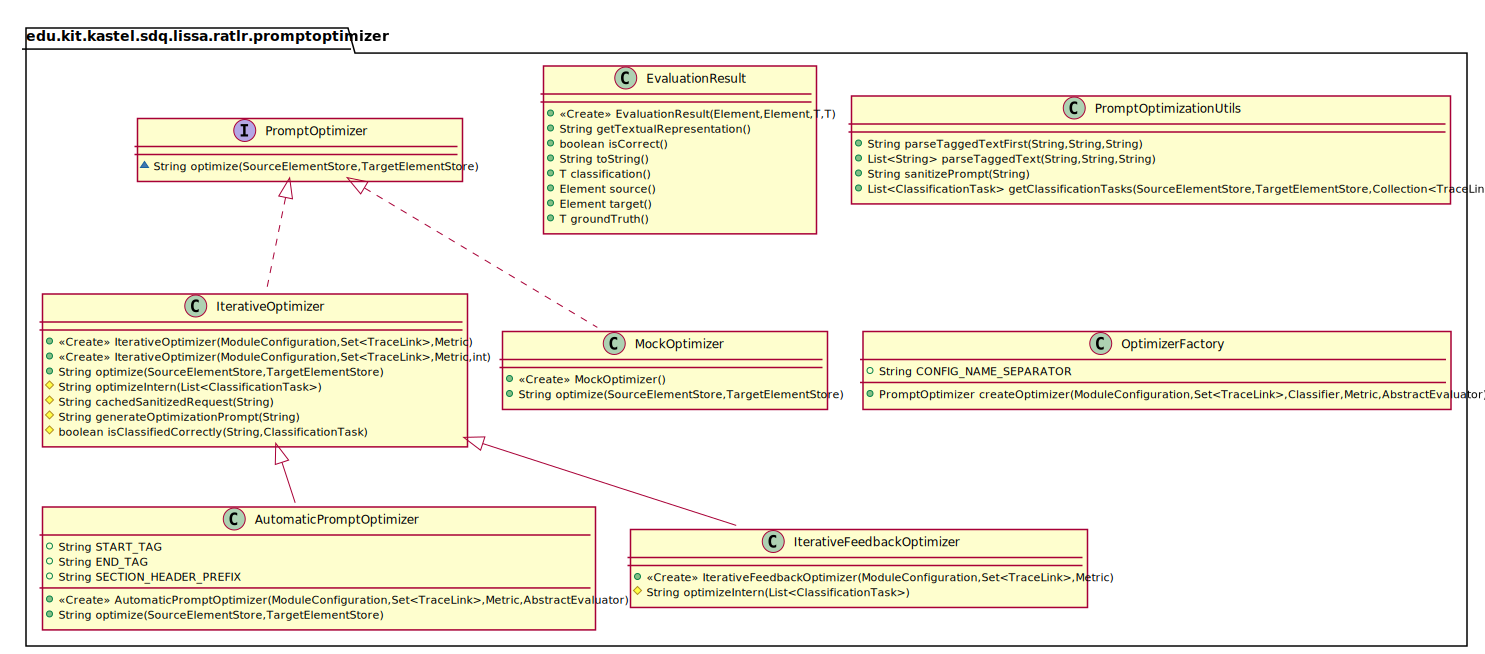
\includegraphics[width=\textwidth]{graphics/class_diagrams/optimizer}
    \caption{The new \promptoptimizer component and its implementations}
    \label{fig:optimizer_component_diagramm}
\end{figure}

As seen in \autoref{fig:optimizer_component_diagramm}, the \promptoptimizer component will typically use the \LLM to evaluate different prompts.
\Todo{It has not been seen...}

Many implementations of the \promptoptimizer component will require sampling strategies as a heuristic to reduce the number of calls to the \LLM.
\Todo{Is heuristic the right word here?}
The \samplingstrategy subcomponent provides different strategies to select a sublist of comparable elements from a collection.
The strategies can be instantiated with configuration parameters and are used by the \promptoptimizer component.
This way, sampling strategies can be swapped easily without changing the actual optimization logic.
The random sampler uses a fixed random seed to ensure reproducibility of results.

\begin{figure}
    \centering
    \fontsize{8}{10}\selectfont
    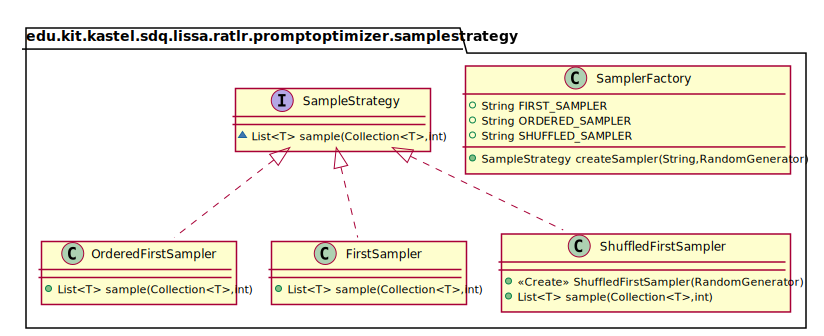
\includegraphics[width=\textwidth]{graphics/class_diagrams/sample_strategy}
    \caption{The new \samplingstrategy subcomponent and its implementations}
    \label{fig:sampling_strategy_diagramm}
\end{figure}

In \autoref{fig:sampling_strategy_diagramm}, the sampling strategy subcomponent is depicted.
Currently, three different strategies are implemented.
\begin{itemize}
    \item The \method{ShuffledFirstSampler} will shuffle the input list using the \method{RandomGenerator} and return the first elements.
    \item The \method{OrderedFirstSampler} will sort the input list and return the first elements.
    \item The \method{FirstSampler} will return the first elements of the input list.
\end{itemize}
\Todo{Nicht nur aufzählen, sondern auch kurz erklären}

\Todo{Alles was in Bilder ist muss beschrieben sein}
\Todo{Zusammenhang zu alten Classifiern muss deutlich erkennbar werden. Fokus dieses ganzen Chapter!}

\section{LiSSA Pipeline Integration}
\label{sec:impl:lissa_integration}
\Todo{Can you use \acs{LiSSA} in the title but without the quote?}
\Todo{Mehr Details, sonst arg kurz}
The new components are integrated into the \LiSSA pipeline.
A new command was added to the \LiSSA command-line interface to run the prompt optimization.
The command will read the configuration file and create the required components using their constructors or factories, respectively.
To do so an evaluation pipeline object is created and relevant components will be retrieved from it.
This includes the classifier, aggregator, trace link id postprocessor as well as the source and target \elementstore's.
The classifier component is used to classify a pair of elements having a \TL or not.

While the optimization pipeline, as a standalone, is independent of the regular evaluation pipeline, they can be combined.
This is achieved by feeding the optimized prompt from the optimization pipeline into the evaluation pipeline, indicated by a separate configuration.
